\section{Background and Related Works}
\label{sec:background}
In this section, we review some issues related to developing an event-based middleware for WSN. We also briefly discuss the works that have done so far to address those issues
We first briefly overview the basic concepts r These concepts will be used extensively when we describe our design for PSWare.

\subsection{WSN-based Middleware}
WSN brings a lot of opportunities as well as some challenges. WSN allows large scale deployment and have a large area of applications. However, developing WSN-based applications is considered challenging because of the following issues.

\emph{Abstraction Support}: WSN usually consists of large number of heterogeneous sensors. These sensors may be developed by different vendors and may have different capability, precision and platform. Therefore, the middleware should hide the underlying platform details and provide a high level programming paradigm for the application programmers. Ideally, a good programming paradigm allows programming the sensor network as a single 'virtual' entity, rather than individual nodes \cite{programmingparadigms}.

\emph{Layered Architecture}: WSN-based middleware offers layered architectures. This is particularly important in WSN enviornment where each sensor node has limited resources like energy, computing power, memory and communication bandwidth. Some middleware provides support to dynamically adapt performance and resource consumption to the varying needs of the application, for example, by enabling dynamic tradeoffs between output quality and resource consumption. Other middleware may need to reliably deliver data over the unreliable wireless links. In addition, multiple applications may run on the same network so the middleware need to fairly assign resources between different applications.

Consequently, a lot of middleware works have been proposed to help on these issues. Existing works on middleware may be categorized according to the programming abstractions they provide including query-based approach, virtual machine-based approach and agent-based approach. Query-based approach views the whole network as a database. The data collected by the sensor nodes are ordered to facilitate the query operations. A representative work in this category is TinyDB \cite{tinydb}.

Agent is another popular programming abstraction for WSN applications. One of the motivations to use agent-based approach is to allow multiple applications to be executed on the same network. Therefore, the codes running on individual sensor nodes are treated as mobile agents and may move between different sensor nodes. A representative work is Agilla \cite{agilla}.

Apart from query and agent, virtual machine is another approach for programming abstraction. In this approach, the middleware provides instruction sets to the upper layer applications. Each instruction is usually linked with an underlying function or handler provided in the middleware. The benefit for such approach is that it is possible to have higher level abstractions on top of the instruction set. For example, a query-based scripting language may be built on top of a VM if the underlying instructions can support query operations effectively. A representative work from this category is Mat\'{e} \cite{mate}.

As discussed in Section \ref{sec:introduction}, many WSN applications are event-based. This may make the query based approach unsuitable for some of the applications since SQL or agent may not be able to express the temporal and spatial relations among different events. In this paper, we propose an event-based middleware named PSWare. Different from the existing event-based middleware, PSWare can support composite events. In addition, PSWare uses a flexible architecture. On the top level, PSWare provides an event definition language which can be used to define composite events. On the lower level, PSWare uses an architecture similar to a virtual machine where different event processing algorithms can be easily integrated by implementing different byte codes.

\subsection{Support of Composite Events}
In this subsection, we overview the event model incorporated by PSWare. In our event model, each event is a list of attributes which are the actual data obtained from the sensor networks. For instance, the temperature and humidity readings in a room can be treated as an event. Events can be primitive or composite. In our event model, primitive events are those that can be directly sensed and obtained by individual sensor nodes.

In practical applications, the user may be only interested in a subset of the events detected by the system. This can be done through event filters (or event subscriptions from the user's point of view). Event filters are constraints applied to individual events. For instance, 'temperature \textgreater 30' may be considered as a filter. Depending on the underlying model, there are mainly three types of subscriptions: content-based, topic-based and type-based \cite{facespubsub}. Continuing with our example, 'temperature \textgreater 30' is content-based filter. If the user is interested in all the humidity readings, then a topic-based subscription can be made which so that the user only subscribes to the humidity readings. 

Compared with topic-based and content-based subscription, type-based subscription is more fine-grained. In this type of subscription, the user first specify the event types. This is similar to defining new types in many programming languages. Since each event is defined as a list of attributes, an event type defines the data types for individual attributes. For example, we can specify a new event type for fire alarm consisting of both humidity and temperature readings. Apart from attribute definition, the event types can also include operators for each attribute. Continuing with our example, we can define the condition for the fire alarm when the temperature reaches a certain threshold while the humidity is below another. 

\begin{figure}
\centering
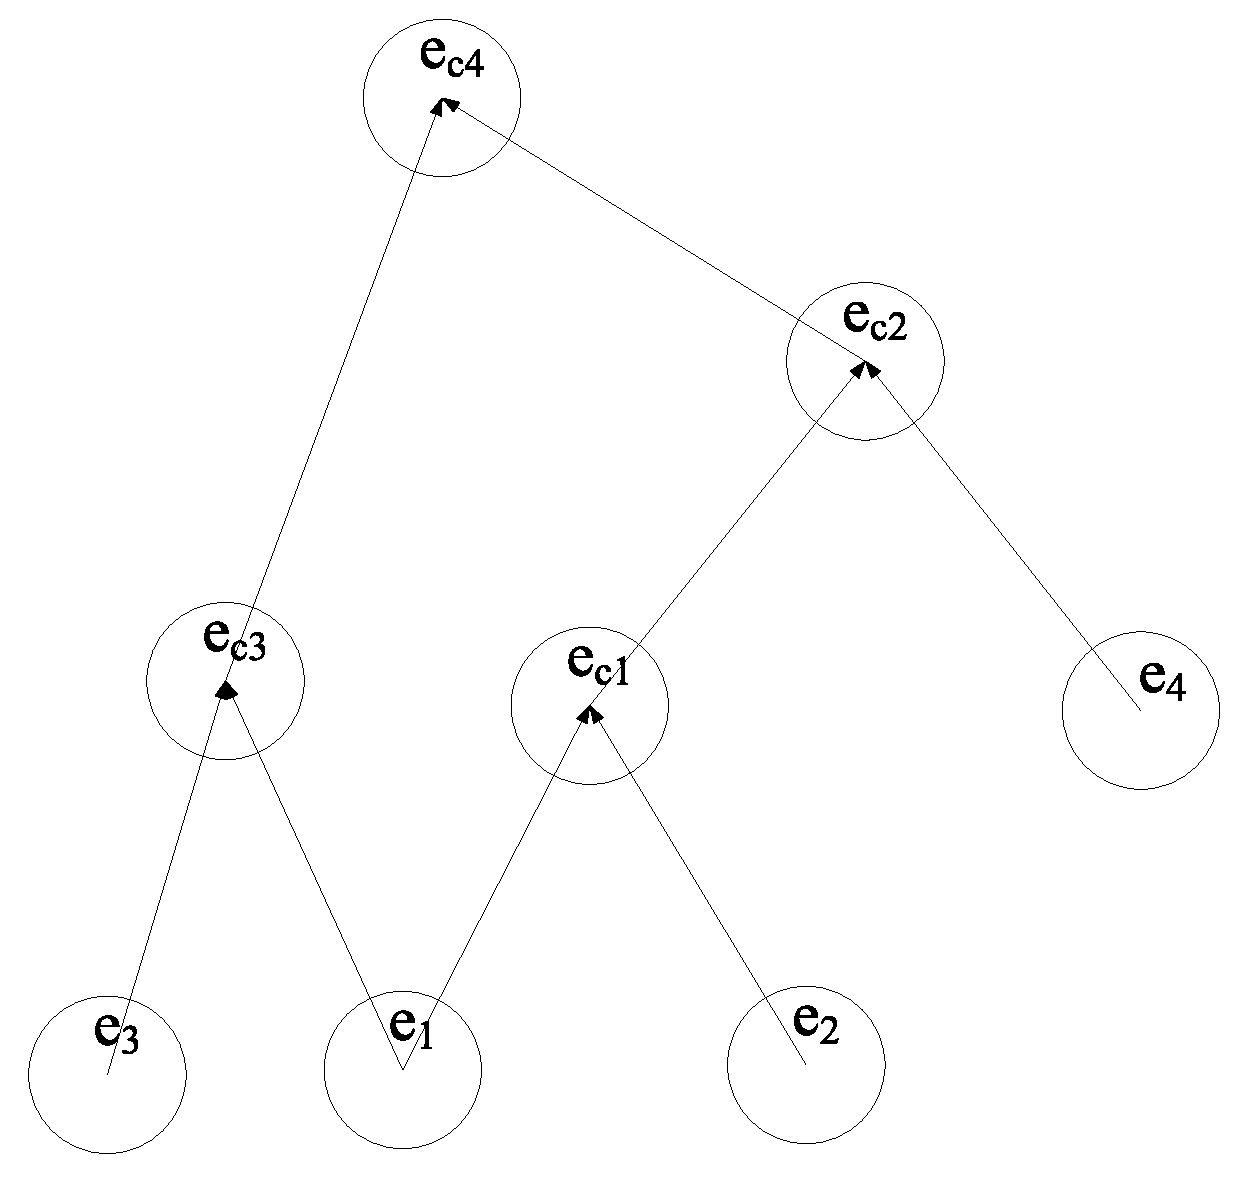
\includegraphics[width=.5\textwidth]{eventhierarchy}
\caption{Event hierarchy}
\label{fig:eventhierarchy}
\end{figure}

In PSWare, we use type-based subscription because composite events can be more easily defined by specifying their types and the corresponding filters. This is similar to many programming languages where composite data types can be defined based on primitive types. The event relations are defined through operators in event filters. For example, we can specify the interval between two events is greater than 10 by writing \(e_1.time - e_2.time > 10\).

Event types together with their relations can be represented as a directed acyclic graph where each node represents an event and the each edge represents a relation. Figure \ref{fig:eventhierarchy} shows an example of such a graph. The nodes with 0 in-degree represent primitive events. The rest of the nodes represent composite events. The event which has 0 out-degree is the subscribed event.

There are a few works for primitive event processing in WSN. However, many of them discuss only primitive events \cite{lowlevelnaming} \cite{directeddiffusion} \cite{mires}. Other works may only emphasize on a specific issue in event processing. For example, \cite{sp} discusses the trade-off between reliability and energy consumption. Instead of propagating the subscription into the whole network, the authors choose to stop forwarding the subscription after a certain number of hops. The publisher will then deliver the events in an opportunistic way. If a node with subscription information is reached, the events will be delivered. Otherwise, the events will be forwarded with a certain probability.

A few recent works such as \cite{lai:ted} \cite{complexevent} have been proposed for composite event definition and detection. The primary focus of \cite{lai:ted} is on a composite event detection algorithm called TED which utilizes event type information for efficient detection. In addition to an event language, \cite{complexevent} also discusses how to reliably detect composite events in a pervasive environment. Different from the previous works, the focus of this paper is on a flexible middleware framework so that different event detection algorithms may be integrated and evaluated easily.

\begin{comment}
\subsection{Composite Event Detection}
If we take the event relations into consideration while detecting the events, then detection can be done with different strategies. In this paper, we mainly consider message cost as event detection cost. Furthermore, since primitive event can be detected by individual sensor nodes, we mainly consider the composite event detection cost in this paper.

In general, if a composite event is detected based on two sub-events \(e_1\) and \(e_2\) as shown in Figure \ref{fig:event-detection2} then the cost for detecting the composite event will be the cost for detecting each individual events together with the cost for delivering the event detection results to the event detector. An event detector here is simply a node responsible for detecting composite events.

\begin{figure}
\centering
\subfloat[Basic composite event detection]{\label{fig:event-detection2}\figurehalfwidth{event-detection2}}
\subfloat[Composite event detection using event probability]{\label{fig:event-detection3}\figurehalfwidth{event-detection3}}
\caption{Composite event detection}
\label{fig:event-detection}
\end{figure}

Sometimes the events may have dependency and certain events must happen before others. In this case, we don't need to make all sensor nodes monitor the events at all the time. Instead, some nodes may firstly put to sleep mode and then be waken up when other events occur. For example, as shown in Figure \ref{fig:event-detection3}, if we have two events \(e_1\) and \(e_2\) which have a relation such that the composite event happens only when both events have been successfully detected. If \(e_2\) and \(e_1\) need to satisfy a relation such that \(e_2\) happens after \(e_1\). Then originally the nodes responsible for monitoring \(e_2\) may be put to sleep mode. After \(e_1\) has successfully been detected, a message can be forwarded to the nodes responsible for detecting \(e_2\) and wake them up. In this way, we can further reduce the energy cost because \(e_2\) doesn't have to be monitored if \(e_1\) doesn't occur.
\end{comment}

\subsection{Flexible Middleware Design}
Flexibility in middleware is mainly achieved by layering so that changes made in one layer will not affect others. In this section, we focus two layers which are of particular interest: the abstraction layer and the data processing layer \cite{layeredDesign}. The reason why these two layers are important to middleware design is:
\begin{itemize}
\item The abstraction layer defines how middleware users can interact with the middleware service and what functionalities the users can have
\item The data processing layer is important because it is challenging to manage the resources in WSN where the sensors have limited capability and communications are expensive and unreliable.
\end{itemize}

In the previous sub-section, we have already discussed some programming abstractions such as database, query and mobile agent supported by existing WSN middleware. Apart from these works, there are other works that discuss programming abstractions. SNAK (Sensor Network Application Construction Kit) \cite{snack} provides high level abstractions in terms of services. A distinct feature of SNACK is that it divides the WSN application programmers into three types. System programmers use NesC to develop reusable components. Service programmers combine those components into services that implement high-level semantics such as routing tree, periodic sensing, etc. Application programmers select a handful of services to run on a given network. By doing so, SNACK effectively provides greater flexibility through layering and allows components reuse.

However, SNACK is different from the middleware works in the previous section in the sense that in SNACK, the high-level script language is converted directly into NesC codes and then compiled into native binaries. However, in middleware works such as Mat\'{e} and Agilla, the middleware runtime environment are pre-installed on each sensor nodes. Then the high level script language are usually translated into the byte codes that can be interpreted by such runtime environment instead of the native binaries. The benefit of using such intermediate layer of byte code is to save communication cost because those byte codes can be application-specific and perform a lot of complicated operations. As a result, the program size maybe reduced if some of the underlying functions are built into the middleware.

Some works use neighbor-based abstractions and Hood \cite{hood} is a representative work. On the high level, it provides the abstraction for finding neighbors and setting / filtering attributes without worrying about where the actual data are stored. Similar to SNACK, Hood will automatically generate the codes into NesC programs and then compile them into native binaries. Hood effectively hides the communication from application developer and makes developing WSN applications easier. Hood also has a several layers for code generation, data caching and data transmission. Because of this, Hood is also quite flexible in the sense that changes in any of those layers will not affect other layers. However, one limitation of Hood is that it can potentially introduce high message cost by broadcast.

In terms of data processing, there are quite a few works in this area, especially for data aggregation. Existing data aggregation can be mainly divided into three categories: cluster-based approach, \cite{leach} \cite{iheed}, chain-based approach \cite{pegasis} and tree-based approach \cite{mfst} \cite{dctc}. Cluster-based approach typically considers the problem how to select and rotate cluster heads so that the clusters can be evenly distributed in the network  and energy consumption will be balanced. A representative work is iHeed \cite{iheed}. Cluster-based approach can be organized into multiple levels in order to further save the cost.

Chain-based approach improves cluster-based approach by letting each sensor node only communicate with its close neighbors. The resulting problem is indeed very similar to traveling sales person problem. PEGASIS \cite{pegasis} is a representative work. Tree-based approaches utilize many techniques from graph theory and perform optimization. For example, \cite{xue:lp} formulates the problem as a multi-commodity flow problem and uses linear programming to solve it.  MFST \cite{mfst} constructs a minimum Steiner tree with a cost model that considers the fusion cost.

Most of the existing works in data aggregation, however, talks mainly about how to use optimization techniques to minimize the underlying communication cost. Little have been mentioned about how these techniques can be easily integrated with the user's applications.